\documentclass{standalone}
% fonts
\usepackage{mathpazo} % math & rm
\linespread{1.05} % Palatino needs more leading (space between lines)
% tikz
\usepackage{tikz}
%\usetikzlibrary{...}
\begin{document}
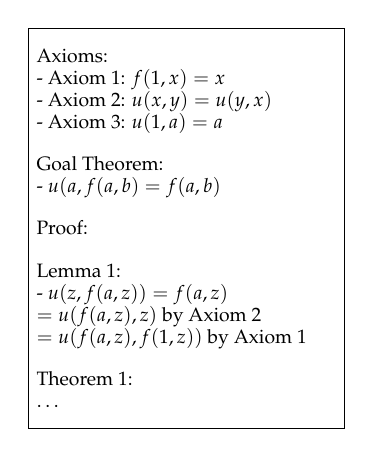
\begin{tikzpicture}
\node[draw,rectangle,inner sep=3pt,minimum height=2in] at (0,0) {%
   \scriptsize%
   \begin{minipage}[b]{1.5in}
      Axioms:\\
      - Axiom 1: $f(1,x) = x$ \\
      - Axiom 2: $u(x,y) = u(y,x)$ \\
      - Axiom 3: $u(1,a) = a$
      \vspace{0.1in}
      
      Goal Theorem: \\
      - $u(a, f(a,b) = f(a,b)$
      \vspace{0.1in}
      
      Proof:
      \vspace{0.1in}
      
      Lemma 1: \\
      - $u(z, f(a,z)) = f(a,z)$ \\
      $= u(f(a,z),z)$ by Axiom 2 \\
      $= u(f(a,z), f(1,z))$ by Axiom 1
      \vspace{0.1in}
      
      Theorem 1: \\
      $\dots$
   \end{minipage}%
};
\end{tikzpicture}%
\end{document}
